\section{ХОД РАБОТЫ}

\subsection{Формулировка задачи}

Для \textit{нормального} и \textit{равномерного} распределения необходимо
вывести в одно графическое окно два графика плотности вероятности. Один из графиков
плотности вероятности получить по собственной программе, написанной для расчета
значений плотностей вероятности, второй --- с использованием функций системы Matlab.

\subsection{Теоретические сведения}

Плотность вероятности при \textit{равномерном} распределении $ U(a,b) $:
$$
  f_{\xi}(x) =  \left\{
                \begin{aligned}
                  \dfrac{1}{b-a}&, &a<x<b \\
                  0&,              &x \le a, x \ge b
                \end{aligned}
                \right.
                , a,b \in R, a<b.
$$

Плотность вероятности \textit{нормального} распределении $ N(a, \sigma^2) $:
$$
  f_{\xi}(x) = \dfrac{1}{\sqrt{2\pi\sigma^2}}*e^{\dfrac{(x-a)^2}{2\sigma^2}}, a \in R, \sigma^2 > 0.
$$

\subsection{Плотность вероятности равномерного распределения}

В системе Matlab определим функцию \textbf{uniform}, используемую для построения
графика \textit{равномерной} плотности вероятности.

\begin{lstlisting}
  function y = uniform(x,a,b)

  y = zeros(size(x));
  distrib_value = 1 ./(b-a)

  k = find(x >= a & x <= b & a < b)

  y(k) = distrib_value
\end{lstlisting}

Построим график плотности вероятности для \textit{равномерного} распределения,
полученный по собственной программе, а затем с использованием библиотечных функций.
Для этого в системе Matlab напишем следующие команды:

\begin{lstlisting}
  a_1 = 3  b_1 = 7
  a_2 = 4  b_2 = 6
  X = 0: 0.1 : 10

  hold on
  % plot(X, unifpdf(X, a_1, b_1))
  % plot(X, unifpdf(X, a_2, b_2))

  plot(X, uniform(X, a_1, b_1), 'r')
  plot(X, uniform(X, a_2, b_2), 'r')
\end{lstlisting}

\begin{figure}[h]
  \begin{minipage}[h]{0.47\linewidth}
    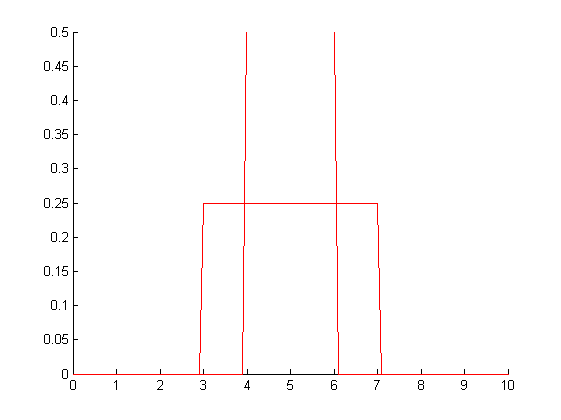
\includegraphics[width=1\linewidth]{pic/uniform_our}
    \caption{График плотности вероятности равномерного распределения, полученный по собственной программе}
  \end{minipage}
  \hfill
  \begin{minipage}[h]{0.47\linewidth}
    \vspace{4mm}
    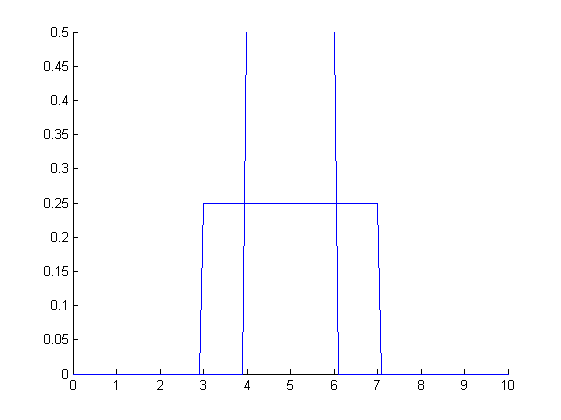
\includegraphics[width=1\linewidth]{pic/uniform_lib}
    \caption{График плотности вероятности равномерного распределения, полученный с помощью библиотечной функции \textbf{unifpdf($x,a,b$)}}
  \end{minipage}
\end{figure}

Стоит отметить, что параметры $a, b$ влияют на <<ширину>> графиков.

\subsection{Плотность вероятности нормального распределения}

В системе Matlab определим функцию \textbf{norm\_pdf}, используемую для построения
графика \textit{нормальной} плотности вероятности.

\begin{lstlisting}
  function y = norm_pdf(x,a,s)
  y = zeros(size(x))
  for i = 1:numel(y)
      y(i) = 1./ sqrt(2*pi*s.^2)*exp(-((x(i)-a).^2)./(2.*s.^2))
  end
\end{lstlisting}

Построим график плотности вероятности для \textit{нормального} распределения,
полученный по собственной программе, а затем с использованием библиотечных функций.
Для этого в Matlab напишем следующие команды:

\begin{lstlisting}
  a_1 = 5   s_1 = 3
  a_2 = 5   s_2 = 7
  X = -30: 0.1 : 35
  % plot(X, normpdf(X, a_1, s_1))
  % plot(X, normpdf(X, a_2, s_2))
  plot(X, norm_pdf(X, a_1, s_1), 'r')
  plot(X, norm_pdf(X, a_2, s_2), 'r')
\end{lstlisting}

\begin{figure}[h]
  \begin{minipage}[h]{0.47\linewidth}
    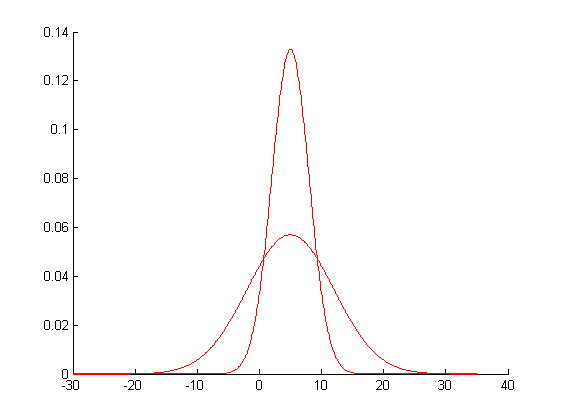
\includegraphics[width=1\linewidth]{pic/norm_our}
    \caption{График плотности вероятности \textit{нормального} распределения, полученный по собственной программе}
  \end{minipage}
  \hfill
  \begin{minipage}[h]{0.47\linewidth}
    \vspace{4mm}
    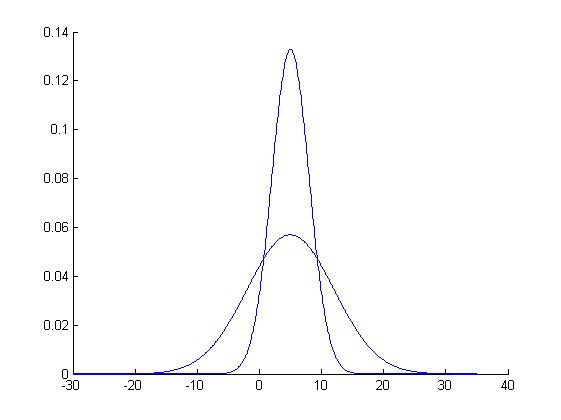
\includegraphics[width=1\linewidth]{pic/norm_lib}
    \caption{График плотности вероятности \textit{нормального} распределения, полученный с помощью библиотечной функции \textbf{normpdf($x,a,\sigma$)}}
  \end{minipage}
\end{figure}

Параметр $a$ функции \textbf{normpdf} влияет на сдвиг графика относительно оси ординат,
параметр $\sigma$ --- на <<вытянутость>> графика.
 
\newpage
